\section{A restriction bound independent of clause count}
\label{sec:restriction}

A random restriction need not reduce every clause of a large CNF to small
width.  The following lemma instead expresses the restricted formula as a
signed combination of small-width tests.  The total absolute coefficient
mass has bounded expectation, regardless of the number of clauses.  The
normalization by counts of violated clauses is what makes this possible.
This is a different conclusion from the classical switching estimate,
which also has no clause-count parameter but changes the formula's
normal form~\cite[Section~3, Main Lemma]{H89}.  Here the tests remain CNFs;
the cost is their signed coefficient mass, controlled in expectation.

\begin{lemma}[Restriction bound]\label{lem:restriction}
Let $k\geq0$ and $b\geq1$ be integers, let $H$ be a CNF of width at most
$k$ on $[d]$, and let $0<p<1$.  Choose $T\subseteq[d]$ by retaining each
coordinate independently with probability $p$, and choose a uniform
assignment $\rho$ outside $T$.  Suppose
\begin{equation}\label{eq:restriction-theta}
  \theta=\sum_{\ell=b+1}^{k}\binom{k}{\ell}
                  \left(\frac{2p}{1-p}\right)^{\ell}<1.
\end{equation}
There are numbers $W(H,T,\rho)\geq 0$, depending only on the formula and
the restriction, such that
\begin{equation}\label{eq:restriction-cost}
  \E_{T,\rho}W(H,T,\rho)\leq\frac{1}{1-\theta}
\end{equation}
and, simultaneously for every real-valued function $G$ on $\bits^T$,
\begin{equation}\label{eq:restriction-correlation}
  \abs{\E_z G(z)H_{T,\rho}(z)}
       \leq W(H,T,\rho)\,\corr_b(G).
\end{equation}
An empty sum in \eqref{eq:restriction-theta} is zero.
\end{lemma}

\begin{proof}
Discard true and tautological clauses from $H$, and list the remaining
clauses as $C_1,\ldots,C_N$, retaining their indices even if clauses repeat.
Let $E_i\subseteq[d]$ be the scope of $C_i$.  Thus $|E_i|\leq k$ and violation
of $C_i$ prescribes one pattern on $E_i$.  A false clause has empty scope
and is always violated.  All sums and families below are finite; there is
no restriction on the finite number $N$.

\medskip\noindent
\textit{Building the finite expansion.}
Fix $T,\rho$, and write $v_i(z)$ for the violation indicator of $C_i$
under this restriction.  Put $q=\sum_i v_i$.  For $U\subseteq T$, define
\begin{equation}\label{eq:restriction-counts}
  a_U=\sum_{i:\,|E_i\cap(T\setminus U)|\leq b}v_i,
  \qquad
  c_U=\sum_{i:\,E_i\cap(T\setminus U)=\varnothing}v_i.
\end{equation}
Call an index \emph{easy at $U$} if it occurs in the first sum, and
\emph{hard at $U$} otherwise.  Once the coordinates in $U$ are prescribed,
an easy clause has at most $b$ variables still free.  The classifications
depend only on scopes, not on the values of $z$.  In particular,
\[
  K=\one[a_{\varnothing}=0]
\]
is the width-at-most-$b$ CNF obtained by conjoining the initially easy
clauses after substituting $\rho$.

We will correct $K$ to obtain $H_{T,\rho}$.  They already agree where
$K=0$ and where $q=0$.  At a point with $K=1$ and $q>0$, however,
$K-H_{T,\rho}=1$, and every violated clause is initially hard.  Dividing
this unit excess among the violated clauses gives
\[
  1=\sum_{i\text{ hard at }\varnothing}\frac{v_i}{q}.
\]
The next step replaces the common denominator $q$ by counts of easy
clauses.  This produces further corrections, indexed by paths of
successive clause violations.

A path $P=(i_1,\ldots,i_j)$ starts with $U_0=\varnothing$ and satisfies
\begin{equation}\label{eq:restriction-path}
  i_h\text{ hard at }U_{h-1},
  \qquad U_h=U_{h-1}\cup(E_{i_h}\cap T)
  \quad(1\leq h\leq j).
\end{equation}
Write $\mathcal P_j(T)$ for the family of these indexed paths.
Each step adds at least $b+1$ coordinates, so their lengths are bounded
by $L=\floor{|T|/(b+1)}$.  The selected indices are distinct: once an
index is selected, its whole live scope belongs to $U_h$, and it stays
easy thereafter.  If all selected clauses are violated, their first
$h$ indices are counted in $c_{U_h}$, and hence
\begin{equation}\label{eq:restriction-positive-count}
  a_{U_h}\geq c_{U_h}\geq h.
\end{equation}
Throughout this expansion, a path fraction is defined to be zero when
its numerator vanishes.  The displayed bound makes every denominator
positive on the numerator's support.

Continue to work at a point with $K=1$ and $q>0$.  For a nonempty path
$P=(i_1,\ldots,i_j)$, distinguish its remaining correction
\[
  r_P=\frac{\prod_{h=1}^{j}v_{i_h}}
             {q\prod_{h=1}^{j-1}a_{U_h}}
\]
from the contribution obtained by replacing the remaining factor $q$
in its denominator with $a_{U_j}$:
\[
  t_P=\frac{\prod_{h=1}^{j}v_{i_h}}
             {\prod_{h=1}^{j}a_{U_h}}.
\]
Since $q=a_{U_j}+\sum_{i\text{ hard at }U_j}v_i$, this replacement gives
\begin{equation}\label{eq:restriction-residual}
  r_P=t_P-\sum_{i\text{ hard at }U_j}r_{Pi},
\end{equation}
where $Pi$ denotes extension by $i$.  Indeed, on the support of the
prefix numerator, the sum over extensions is
$t_P(q-a_{U_j})/q$, leaving $t_Pa_{U_j}/q=r_P$.
If the prefix numerator vanishes, all extension numerators vanish too,
so the identity still holds.

Initially $\sum_{P\in\mathcal P_1(T)}r_P=1$.  Substituting
\eqref{eq:restriction-residual} repeatedly gives, for $0\leq s\leq L$,
\[
  0=1+\sum_{j=1}^{s}(-1)^j\sum_{P\in\mathcal P_j(T)}t_P
       +(-1)^{s+1}\sum_{P\in\mathcal P_{s+1}(T)}r_P.
\]
At $s=L$ there are no further paths, so the residual sum is empty.
Together with the cases $K=0$ and $q=0$, this proves the pointwise identity
on the whole live cube
\begin{equation}\label{eq:restriction-expansion}
 H_{T,\rho}
   =K+K\sum_{j=1}^{L}(-1)^j
          \sum_{P\in\mathcal P_j(T)}
          \frac{\prod_{h=1}^{j}v_{i_h}}
               {\prod_{h=1}^{j}a_{U_h}}.
\end{equation}
The construction is finite; no convergence argument is involved.

\medskip\noindent
\textit{Each path is a positive weight times a finite convex mixture.}
A path is \emph{compatible} with $\rho$ if all its selected clauses can
be violated simultaneously.  Such violations prescribe exactly one
pattern $\sigma_P\in\bits^{U_j}$, with no conditions on $T\setminus U_j$.
Indeed, each selected clause prescribes its unique violating pattern;
compatibility says that the prescriptions agree on overlaps and with
$\rho$.  Write
\[
  \mathcal Z_P=\{z\in\bits^T:z|_{U_j}=\sigma_P\}
\]
for this cylinder.  Then $\prod_hv_{i_h}=\one_{\mathcal Z_P}$.  An
incompatible path has zero numerator everywhere and can be omitted.

For a compatible path and each $h$, the function $c_{U_h}$ is constant on
$\mathcal Z_P$.  Every clause in its defining sum uses only coordinates
already fixed by $\rho$ and the pattern on $U_h$.  Denote this positive
integer constant by $c_h$, and set
\begin{equation}\label{eq:restriction-path-weight}
    \omega(P)=\prod_{h=1}^{j}\frac{1}{c_h}.
\end{equation}
On $\mathcal Z_P$ we have $a_{U_h}=c_h+w_h$, where
\[
 w_h=\sum_{i\in I_h}v_i,
 \qquad
 I_h=\{i:0<|E_i\cap(T\setminus U_h)|\leq b\}.
\]
Substitute both $\rho$ and the final pattern $\sigma_P$ into each clause
indexed by $I_h$.  The resulting clauses on $T\setminus U_j$ have width
at most $b$, since $U_h\subseteq U_j$.  Keep their original indices in this
family, including clauses that become true or false and any repetitions.
Thus $w_h$ remains exactly the number of violated clauses in this indexed
family, even when some violations become constant after the final
substitution.

We use the following elementary finite mixture.  Given an indexed family
of $a$ clauses and an integer $c\geq1$, uniformly permute the $a$ clause objects
and $c$ distinct marker objects.  Take the conjunction of the clauses
appearing before the first marker.  This finite uniform experiment
defines a convex mixture of conjunctions of the indexed clauses.
If an assignment violates exactly $w$ of the indexed clauses, the sampled
conjunction holds precisely when the first object among those $w$ clauses
and the $c$ markers is a marker.  By symmetry its expectation is
\begin{equation}\label{eq:restriction-mixture-ratio}
       \frac{c}{c+w}.
\end{equation}
The argument includes $a=0$, $w=0$, repeated clauses, and constant clauses.

Independently apply this mixture at each $h$ to the reduced clauses
indexed by $I_h$, with $c=c_h$.  Form $J_P$ by conjoining all sampled
clauses, $K$, and the unit clauses prescribing $\sigma_P$ on $U_j$.
Every realization of $J_P$ lies in $\mathcal C_b(T)$; here the assumption
$b\geq1$ permits the unit clauses.  On the cylinder the independent
mixtures have expected product $\prod_h c_h/(c_h+w_h)$, while off the
cylinder $J_P$ vanishes.  Consequently, as functions on the entire live
cube,
\begin{equation}\label{eq:restriction-path-mixture}
   K\frac{\prod_{h=1}^{j}v_{i_h}}
           {\prod_{h=1}^{j}a_{U_h}}
          =\omega(P)\,\E[J_P].
\end{equation}
The expectation here is over a finite auxiliary probability space.  It
does not involve the test function $G$.

Define $W_0(H,T,\rho)=1$, and, for $j\geq1$, let
\begin{equation}\label{eq:restriction-W}
 W_j(H,T,\rho)=
      \sum_{\substack{P\in\mathcal P_j(T)\\P\text{ compatible with }\rho}}
                \omega(P),
 \qquad
 W(H,T,\rho)=\sum_{j=0}^{\floor{d/(b+1)}}W_j(H,T,\rho).
\end{equation}
For each fixed restriction, combine \eqref{eq:restriction-expansion} and
\eqref{eq:restriction-path-mixture}, then take the correlation with $G$
and use the triangle inequality.  Since $K$ and every realization of every
$J_P$ have width at most $b$, this gives
\eqref{eq:restriction-correlation}.  Both $W$ and all the mixtures were
chosen without reference to $G$, so the inequality holds simultaneously
for every real-valued $G$.

\medskip\noindent
\textit{Reweighting by a full assignment.}
It remains to bound $\E W_j$.  Generate a uniform full assignment
$y\in\bits^d$ independently of $T$, and set $\rho=y|_{[d]\setminus T}$.
This gives exactly the required distribution of restrictions.
Conditional on $T,\rho$, the live part of $y$ is uniform.  For a compatible
path $P$, it lies in $\mathcal Z_P$ with probability $2^{-|U_j|}$; on that
event every selected clause is violated and every $c_{U_h}$ equals $c_h$.
Thus, conditional on each $T,\rho$, multiplying by $2^{|U_j|}$ exactly
undoes the probability of its cylinder.  In particular,
\begin{equation}\label{eq:restriction-full-assignment}
 \E_{T,\rho} W_j(H,T,\rho)
  =\E_{T,y}\!\left[
      \sum_{\substack{P\in\mathcal P_j(T)\\
                      C_{i_1},\ldots,C_{i_j}\text{ violated at }y}}
        2^{|U_j|}\prod_{h=1}^{j}\frac{1}{c_{U_h}(y|_T)}
                 \right].
\end{equation}
The identity holds separately for every path before summing.  It does not
assume that compatibility or the denominator counts are independent of
the restriction.

\medskip\noindent
\textit{Counting paths backwards.}
Fix $y$.  For $R\subseteq[d]$, let
\[
   V_R=\{i:C_i\text{ is violated at }y,\ E_i\cap R=\varnothing\}.
\]
For a path counted in \eqref{eq:restriction-full-assignment}, put
\begin{equation}\label{eq:restriction-reverse-state}
   D_h=U_h\setminus U_{h-1},\qquad
   R_h=T\setminus U_h \quad(0\leq h\leq j),
\end{equation}
where $D_h$ is used only for $h\geq1$.  These sets satisfy
\begin{equation}\label{eq:restriction-reverse-properties}
  i_h\in V_{R_h},\quad D_h\subseteq E_{i_h},\quad |D_h|>b,
  \quad R_{h-1}=R_h\mathbin{\dot\cup}D_h,
  \quad c_{U_h}(y|_T)=|V_{R_h}|.
\end{equation}
In particular, all displayed denominator counts are positive.
Figure~\ref{fig:reverse-paths} depicts how a forward step removes $D_h$
from the live remainder and a reverse step adds it back.

\begin{figure}[htbp]
\centering
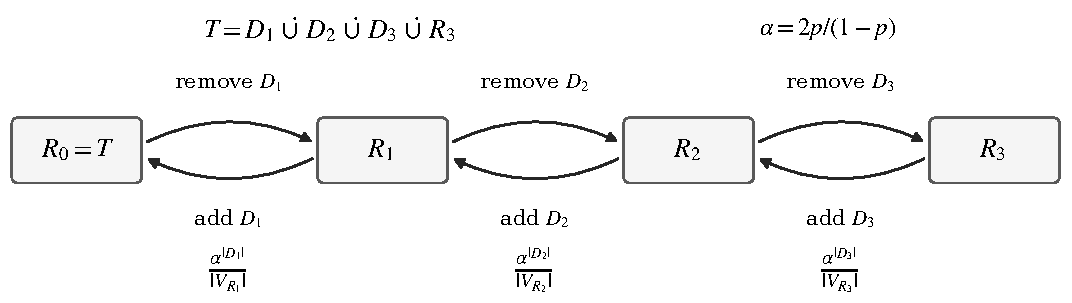
\includegraphics[width=\textwidth]{figures/reverse_paths.pdf}
\caption{A schematic three-step path for a fixed full assignment \(y\),
with clause indices suppressed.  Forward steps remove newly prescribed
coordinates from the live remainder.  Each reverse arrow chooses
\((i_h,D_h)\) and adds \(D_h\) to \(R_h\).  The factor
\(1/|V_{R_h}|\) averages over eligible violated clause indices at its
source state \(R_h\), cancelling their number in the one-step estimate.}
\label{fig:reverse-paths}
\end{figure}

The pair consisting of $T$ and its indexed path is determined by the
terminal set $R_j$ and the successive reverse choices
$(i_j,D_j),\ldots,(i_1,D_1)$.  Indeed, each choice reconstructs
$R_{h-1}=R_h\cup D_h$, recovering $T=R_0$ and every selected index.
It is therefore enough to count reverse sequences starting from an
arbitrary set $R$, allowing a choice of any $i\in V_R$ and any
$D\subseteq E_i$ with $|D|>b$, followed by the state $R\cup D$.
Because $E_i\cap R=\varnothing$, this step always adds $D$ disjointly.
All actual reversed paths are included, and allowing additional sequences
can only increase a sum of nonnegative weights.

Write
\[
   \alpha=\frac{2p}{1-p},\qquad
   \pi(R)=p^{|R|}(1-p)^{d-|R|}.
\]
The sets $D_1,\ldots,D_j$ partition $U_j$, and $T=R_j\mathbin{\dot\cup}U_j$.
The contribution of a given pair $(T,P)$, including the probability of its
live set, therefore factors as
\begin{equation}\label{eq:restriction-reverse-weight}
  \pi(T)\,2^{|U_j|}\prod_{h=1}^{j}\frac{1}{c_{U_h}(y|_T)}
     =\pi(R_j)\prod_{h=1}^{j}
            \frac{\alpha^{|D_h|}}{|V_{R_h}|}.
\end{equation}
This formula explains the useful direction of counting: at state $R$,
the reciprocal count is exactly $1/|V_R|$, the normalization for averaging
over the possible clause indices at that state.

For completeness, define the total weight of $s$ reverse steps from $R$
recursively by $F_0(R)=1$ and
\begin{equation}\label{eq:restriction-reverse-recurrence}
 F_s(R)=
 \begin{cases}
 \displaystyle\frac{1}{|V_R|}\sum_{i\in V_R}
         \sum_{\substack{D\subseteq E_i\\|D|>b}}
                 \alpha^{|D|}F_{s-1}(R\cup D),&V_R\ne\varnothing,\\[3mm]
 0,&V_R=\varnothing,
 \end{cases}
 \qquad(s\geq1).
\end{equation}
The total weight of the choices at a state with $V_R\ne\varnothing$ is
\begin{align}
 \frac{1}{|V_R|}\sum_{i\in V_R}
             \sum_{\substack{D\subseteq E_i\\|D|>b}}\alpha^{|D|}
   &=\frac{1}{|V_R|}\sum_{i\in V_R}
          \sum_{\ell=b+1}^{|E_i|}\binom{|E_i|}{\ell}\alpha^\ell
       \notag\\
   &\leq\sum_{\ell=b+1}^{k}\binom{k}{\ell}\alpha^\ell
     =\theta.\label{eq:restriction-one-step}
\end{align}
When $V_R$ is empty the total weight is zero.  Induction in
\eqref{eq:restriction-reverse-recurrence} now yields
$F_s(R)\leq\theta^s$ for every $R$ and every fixed $y$.  Notice that
\eqref{eq:restriction-one-step} averages over the clause indices instead
of multiplying by their number.  Repeated clauses cause no difficulty:
their multiplicities occur in both the sum and $|V_R|$.

Use the injective reverse encoding and
\eqref{eq:restriction-reverse-weight} to bound the expectation over $T$
inside \eqref{eq:restriction-full-assignment}, for this fixed $y$, by
\[
      \sum_{R\subseteq[d]}\pi(R)F_j(R)
        \leq\theta^j\sum_{R\subseteq[d]}\pi(R)=\theta^j.
\]
Averaging over $y$ gives $\E W_j\leq\theta^j$.  Finally, all terms are
nonnegative and $\theta<1$, so
\[
  \E W
       \leq\sum_{j=0}^{\floor{d/(b+1)}}\theta^j
       \leq\frac{1}{1-\theta},
\]
as required.  Empty formulas, false clauses, and empty live sets are
already covered by the construction; if $k\leq b$, there are no nonempty
paths and $W=1$.
\end{proof}
